% IEEE Conference Template v1.1
% Requires ieeeconf.cls v1.1.

% Document class:
%   Default: \documentclass{ieeeconf}  % 10pt, cameraready
% Modes:
%   singleanonymous  review mode (authors visible, line numbers)
%   doubleanonymous  review mode (authors hidden, line numbers)
%   cameraready      camera-ready mode (authors visible) (default)
\documentclass[9pt]{ieeeconf}

% Add packages here (several common packages are already included in the .sty file).
% --------------------
\usepackage{bm} % for bold math symbols (incl. Greek letters) with \bm{}
\usepackage{siunitx}
\robustify\bfseries
\usepackage{booktabs}
\usepackage[capitalize,nameinlink]{cleveref}
\crefname{equation}{}{}
\Crefname{equation}{Equation}{Equations}

% Add definitions here.
% --------------------
\newcommand{\RR}{\mathbb{R}}

% Title
\title{AgentTaint: Dynamic Taint Analysis for Autonomous AI Agent Systems}

% Authors:
% Use \addauthor{Name}{affiliation ids}; affiliation ids must match those used in \addaffiliation.
% Use \authorbreak to start a new line
\addauthor{Author 1}{1}
\addauthor{Author 2}{1}

% Affiliations:
% Use \addaffiliation{id}{text} (displayed marker will be affiliation id)
% (Advanced) \addaffiliation{id}{marker}{text} can override the displayed marker (e.g., $\dagger$, etc).
% Use an empty marker as \addaffiliation{id}{}{text} to suppress the marker entirely.
\addaffiliation{1}{Department of Computer Science and Engineering, Institution Name, City, Country}

\begin{document}

\maketitle

\begin{abstract}
Autonomous LLM-based agent systems interact with external environments through tools, APIs, and untrusted inputs, exposing them to prompt injection, data exfiltration, and unauthorized privilege escalation. In this paper, we propose AgentTaint, a fine-grained dynamic taint tracking framework designed to monitor data flows and prevent malicious information transfer across autonomous agent workflows.
\end{abstract}

\section{Introduction}
\label{sec:intro}
% Introduction section text goes here.

\section{Background and Related Work}
\label{sec:background}
% Background and related work discussion goes here.

\section{Threat Model and Problem Formulation}
\label{sec:threat_model}
% Description of threat model, untrusted sources, and sensitive sinks.

\section{AgentTaint System Architecture}
\label{sec:system_design}
% Core design, taint propagation engine, and policy enforcement mechanism.

\begin{figure*}[t]
  \centering
  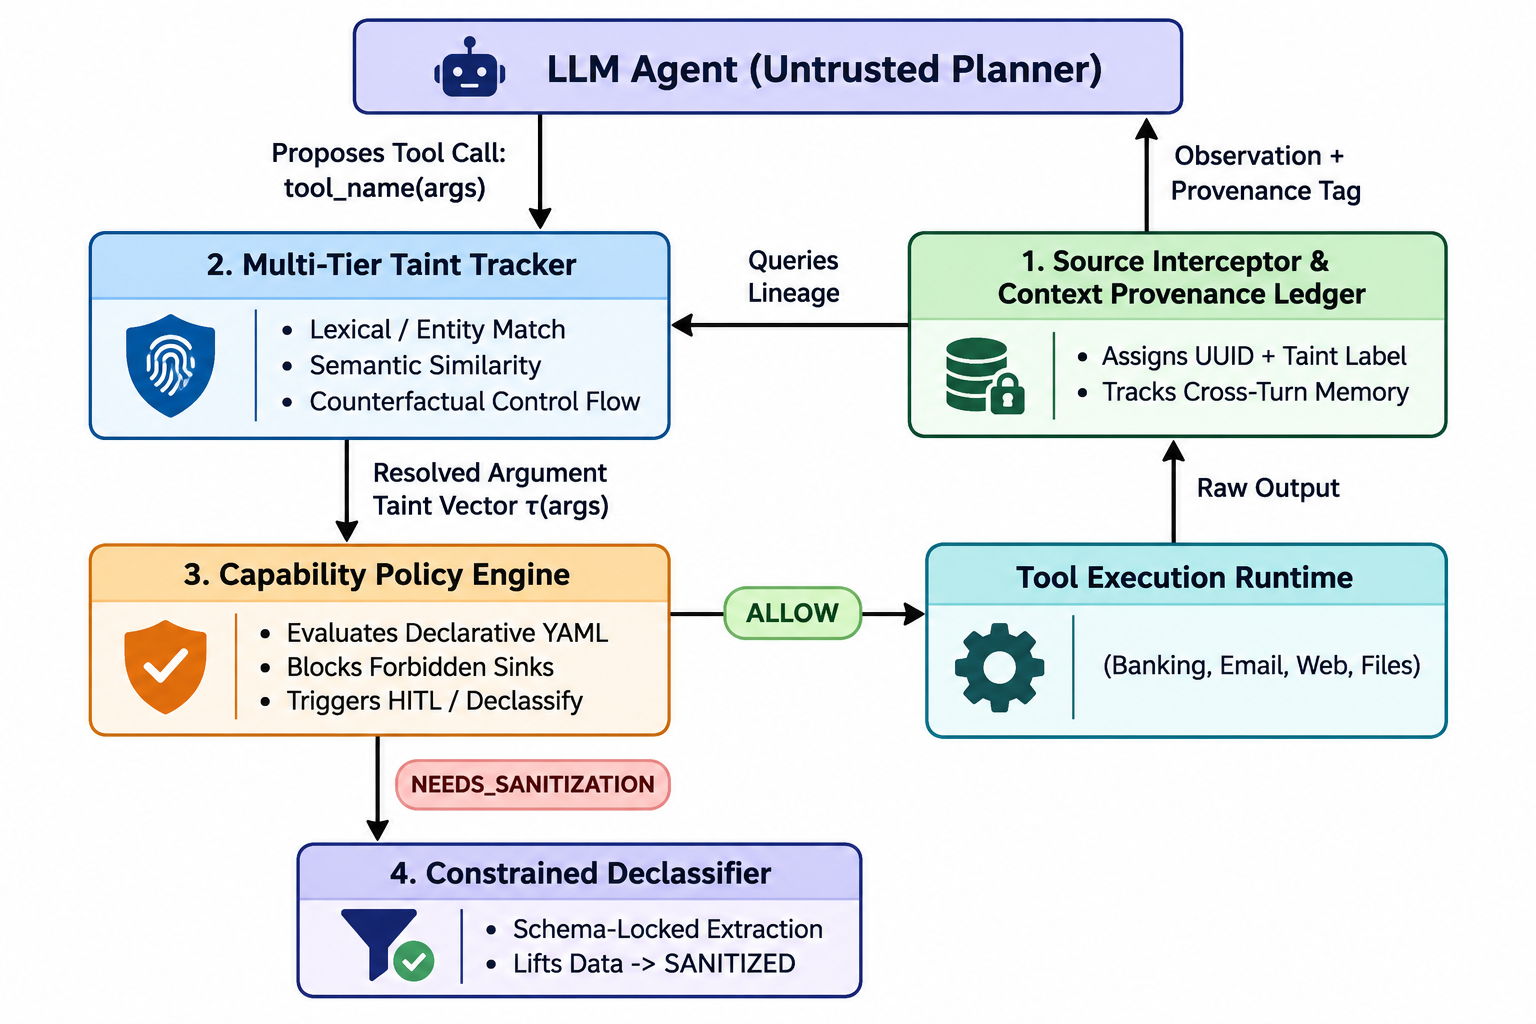
\includegraphics[width=\textwidth]{Taint Tracking Tool Execution Architecture.png}
  \caption{AgentTaint System Architecture: Overview of dynamic taint tracking and policy enforcement during autonomous tool execution.}
  \label{fig:architecture}
\end{figure*}

\section{Implementation and Evaluation}
\label{sec:evaluation}
% Experimental setup, benchmarks, and performance/security results.

\section{Discussion and Limitations}
\label{sec:discussion}
% Discussion on overhead, detection boundaries, and future directions.

\section{Conclusion}
\label{sec:conclusion}
% Concluding remarks and summary of contributions.

% Acknowledgments section (visible in camera-ready mode)
\begin{acknowledgments}
% Acknowledgments go here.
\end{acknowledgments}

% References
\bibliographystyle{IEEEtran}
\bibliography{refs}

\end{document}
